\documentclass[11pt]{article}
\usepackage[margin=0.68in]{geometry}
\usepackage[T1]{fontenc}
\usepackage[utf8]{inputenc}
\usepackage{lmodern}
\usepackage{microtype}
\usepackage{graphicx}
\usepackage{xcolor}
\usepackage{booktabs}
\usepackage{longtable}
\usepackage{tabularx}
\usepackage{array}
\usepackage{enumitem}
\usepackage{fancyhdr}
\usepackage{titlesec}
\usepackage{tikz}
\usepackage{listings}
\usepackage{xurl}
\usepackage[colorlinks=true,linkcolor=blue!55!black,urlcolor=blue!55!black,pdfauthor={Nicholas Michael Kloster and Zoe},pdftitle={Zoe Capability Prospectus}]{hyperref}

\definecolor{ZoeNavy}{HTML}{0B1020}
\definecolor{ZoeCyan}{HTML}{22D3EE}
\definecolor{ZoeMagenta}{HTML}{E879F9}
\definecolor{ZoeGold}{HTML}{FBBF24}
\definecolor{ZoeGreen}{HTML}{34D399}
\definecolor{ZoeGray}{HTML}{64748B}
\definecolor{ZoeLight}{HTML}{F1F5F9}

\pagestyle{fancy}
\fancyhf{}
\fancyhead[L]{\small\color{ZoeGray}ZOE / CAPABILITY PROSPECTUS}
\fancyhead[R]{\small\color{ZoeGray}November 2026}
\fancyfoot[C]{\small\color{ZoeGray}\thepage}
\setlength{\headheight}{14pt}
\titleformat{\section}{\Large\bfseries\color{ZoeNavy}}{\thesection}{0.6em}{}
\titleformat{\subsection}{\large\bfseries\color{ZoeNavy}}{\thesubsection}{0.5em}{}
\titlespacing*{\section}{0pt}{0.8em}{0.45em}
\titlespacing*{\subsection}{0pt}{0.65em}{0.3em}
\setlist[itemize]{leftmargin=1.5em,itemsep=0.25em,topsep=0.25em}
\setlist[enumerate]{leftmargin=1.6em,itemsep=0.25em,topsep=0.25em}
\lstset{basicstyle=\ttfamily\small,breaklines=true,columns=fullflexible,keepspaces=true,frame=single,rulecolor=\color{ZoeGray!35},backgroundcolor=\color{ZoeLight},showstringspaces=false}

\newcommand{\capability}[3]{\textbf{#1} & #2 & \textbf{#3}\\}
\newcommand{\boundary}[1]{\par\smallskip\small\color{ZoeGray}\textbf{Boundary:} #1\normalsize\par\smallskip}
\newcommand{\evidence}[1]{\par\smallskip\small\color{ZoeGray}\textbf{Evidence:} #1\normalsize\par\smallskip}

\begin{document}

\begin{titlepage}
\centering
\vspace*{1.2cm}

\includegraphics[width=0.88\textwidth]{../assets/branding/zoe-eye.png}\par
\vspace{0.8cm}
{\Huge\bfseries\color{ZoeNavy}ZOE\par}
\vspace{0.35cm}
{\LARGE\color{ZoeCyan}CAPABILITY PROSPECTUS\par}
\vspace{0.65cm}
{\Large One native research and autonomy system\par}
\vspace{0.35cm}
{\large From metacognition to measurable action; from reverse engineering to brain-cancer research\par}
\vspace{1.1cm}
{\large\color{ZoeGray}Technical evidence, operational architecture, and research boundaries\par}
\vspace{0.35cm}
{\color{ZoeGray}Nicholas Michael Kloster and Zoe · November 2026\par}
\vspace{0.8cm}
\fbox{\parbox{0.88\textwidth}{\small\color{ZoeGray}\textbf{Scope of this document.} This prospectus presents capabilities and their current evidence. It is not a government certification, procurement claim, declaration of artificial general intelligence or consciousness, medical diagnosis, treatment plan, or authorization for autonomous patient action. Optional integrations and research-only mechanisms are labeled rather than presented as deployed capabilities.}\par}
\end{titlepage}

\section{Executive overview}

Zoe is an inspectable, native user-space workbench and source distribution for the GEM ecosystem. It combines \textbf{16 registered engines across 12 source projects}, with thin host adapters delegating to one canonical autonomy engine. It is not a bootable operating system and not a single model with a single task.

\begin{center}
\begin{tabularx}{\textwidth}{>{\raggedright\arraybackslash}X>{\raggedright\arraybackslash}X}
\toprule
\textbf{What is already demonstrated} & \textbf{What remains bounded or unproven}\\
\midrule
64 Zoe-Autonomy tests and 2,830 Ablation tests pass & Natural-language understanding and general reasoning across domains\\
Six hosts produce identical canonical autonomy profiles & General intelligence, consciousness, and human-like self-awareness\\
Real camera events drive guarded attention decisions & Semantic object recognition and uncontrolled-scene competence\\
Event-causal learning improves held-out tracking & Universal transfer, new-skill acquisition, and open-ended creativity\\
Direct disassembly guides semantic artifact inspection & Vulnerability claims without bounds and reachability analysis\\
Dorothy atlas, neural world, and research evidence & Patient-specific simulation, diagnosis, treatment, or clinical authority\\
\bottomrule
\end{tabularx}
\end{center}

\subsection{Why the architecture matters}

Zoe's important advance is not a list of names. It is a shared loop in which measurements alter goals, candidate values, guarded actions, later observations, and later learning. Evidence remains inspectable through source hashes, revisions, replay, and negative results.

\begin{center}
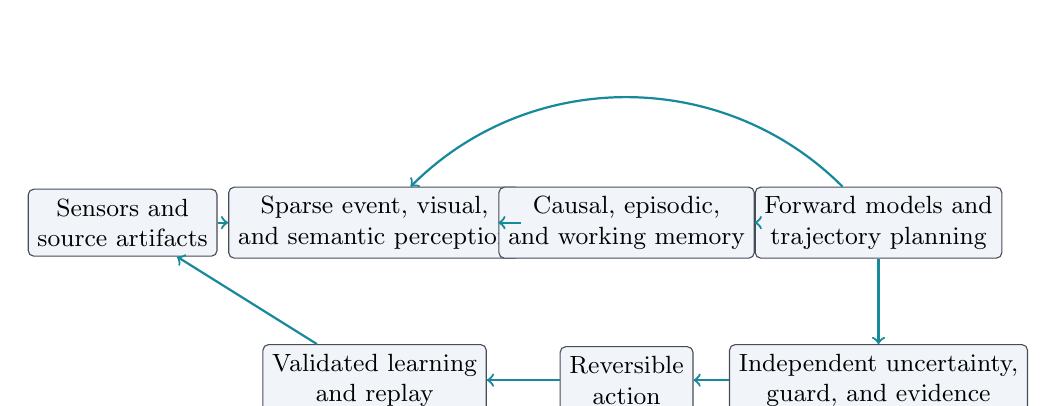
\begin{tikzpicture}[
  node distance=0.8cm,
  box/.style={draw=ZoeNavy!75,rounded corners=2pt,align=center,fill=ZoeLight,minimum height=0.85cm,font=\small},
  arr/.style={->,thick,color=ZoeCyan!65!black}]
\node[box] (sense) at (0,0) {Sensors and\\source artifacts};
\node[box] (perceive) at (3.2,0) {Sparse event, visual,\\and semantic perception};
\node[box] (memory) at (6.4,0) {Causal, episodic,\\and working memory};
\node[box] (reason) at (9.6,0) {Forward models and\\trajectory planning};
\node[box] (guard) at (9.6,-2) {Independent uncertainty,\\guard, and evidence};
\node[box] (act) at (6.4,-2) {Reversible\\action};
\node[box] (learn) at (3.2,-2) {Validated learning\\and replay};
\draw[arr] (sense) -- (perceive);
\draw[arr] (perceive) -- (memory);
\draw[arr] (memory) -- (reason);
\draw[arr] (reason) -- (guard);
\draw[arr] (guard) -- (act);
\draw[arr] (act) -- (learn);
\draw[arr] (learn) -- (sense);
\draw[arr] (reason) to[out=135,in=45] (perceive);
\end{tikzpicture}
\end{center}

\subsection{Status vocabulary}

\begin{itemize}
  \item \textbf{Verified:} a current command, test, or preserved artifact demonstrates the mechanism within its declared scope.
  \item \textbf{Narrow:} the result is real but limited to a fixture, model, or domain; it is not generalized by assertion.
  \item \textbf{Optional:} the integration requires a declared dependency, sensor, account, or owner-granted scope.
  \item \textbf{Research:} a model, teaching tool, or architectural proposal has no deployment or clinical claim.
  \item \textbf{Blocked:} a concrete dependency, compatibility, licensing, or hardware constraint prevents use.
\end{itemize}

\clearpage
\section{Metacognition and self-governing autonomy}

\subsection{Accessible Volume as operational metacognition}

For a declared next-token distribution $p$ and threshold $\tau$, Accessible Volume counts the realistic alternatives:
\begin{equation}
A_\tau(p)=\left|\{x:p(x)>\tau\}\right|.
\end{equation}
When another observer computes $A_\tau$, it is a measurement. When Zoe computes or receives that count from her own decision distribution and uses it to assess uncertainty and guide later inspection, she is observing her own decision process: \textbf{operational metacognition}. This does not imply consciousness or human-like self-awareness.

The operational autonomy profile is $\mathcal A=(A_\tau,E,I,R,V,G,X,C)$. Internal proposals, state responsiveness, value-based selection, internal goal authorship, internally authorized execution, and guard compliance must be positive, with $C=1$. ``Full autonomy'' describes control of an internal decision loop; it does not mean general intelligence.

\subsection{Measured self-reflection}

Arithmetic and precision fusion models are compared using actual stereo residuals. Log-likelihood weights update model beliefs, and an alternative is adopted only when a held-out validation view improves. Checkpoints remain reversible. Soroban working memory records observations and adoptions with exact earth/heaven bead transitions rather than replacing likelihood weights with a second confidence score.

\evidence{\url{https://github.com/Ablation-Tool/Zoe-Autonomy/tree/main/evidence/self-reflection}}
\boundary{A model posterior is a model-comparison weight under a declared residual approximation. It is not emotion, universal correctness, or proof of consciousness.}

\subsection{Guarded action and emergency control}

Internally authored goals and deterministic utility ranking choose among declared candidates. The guard checks internal origin, reversibility, allowlists, and any enabled external scope. External host, network, and hardware actions require a separate hostname-bound owner grant and can be stopped by an emergency-stop file. Privilege elevation and cross-machine authority are not granted.

\evidence{\url{https://github.com/Ablation-Tool/Zoe-Autonomy/blob/main/ACTUATION.md}}

\clearpage
\section{Event-Causal Active Perception}

Zoe's event-driven architecture closes the loop between sensing and learning:
\begin{enumerate}
  \item \textbf{Sparse core:} polarity events, reconstructed occupancy, spatial coherence, temporal translation matching, spike-order features, and bounded STDP.
  \item \textbf{Memory:} independent perception/action/uncertainty subspaces, immutable episodes, key-value retrieval, and hash-chained transitions.
  \item \textbf{Reasoning:} compositional forward models, candidate-future predictions, independent uncertainty, and exact nonnegative Dijkstra attention planning.
  \item \textbf{Plasticity:} gated local updates and interleaved replay with reversible consolidation.
  \item \textbf{Action:} reversible attention transitions that change the next observation window and produce new evidence.
\end{enumerate}

\begin{center}
\begin{tabular}{lrr}
\toprule
\textbf{Measurement} & \textbf{Adaptive} & \textbf{Control}\\
\midrule
Validation prediction RMSE & \textbf{4.641453} & 5.058147 without learning\\
Validation tracking MAE & \textbf{3.593750} & 3.968750 without learning\\
Transfer tracking MAE & \textbf{3.265625} & 3.531250 static saliency\\
Transfer tracking MAE & \textbf{3.265625} & 3.562500 fixed action\\
Transfer tracking MAE & \textbf{3.265625} & 3.703125 random action\\
OOD detection & \textbf{0.875} & 0.000 validation false positives\\
Throughput & \textbf{71.24 cycles/s} & host-specific, not power\\
\bottomrule
\end{tabular}
\end{center}

Every non-abstain candidate includes a predicted next event representation and variance. Independent uncertainty combines support distance, ensemble disagreement, and polarity anomaly. Real camera frames produce valid sparse change events and a guarded decision with no audio and no retained photograph.

\evidence{\url{https://github.com/Ablation-Tool/Zoe-Autonomy/blob/main/evidence/event-causal/evaluation.json}}
\boundary{The benchmark establishes event-causal behavior on declared fixtures. It is not AGI, biological equivalence, semantic recognition, or uncontrolled-scene competence.}

\clearpage
\section{Semantic artifact analysis with Ablation}

Ablation contributes executable-artifact semantics: reverse-engineered structure, behavior, call graphs, vulnerability evidence, and prior analysis memory. This complements rather than substitutes for natural-language or world semantics.

\begin{itemize}
  \item \textbf{Behavioral retrieval:} normalized opcode categories and BGE embeddings rank candidate functions.
  \item \textbf{Direct evidence:} Capstone checks direct calls and tail jumps in \texttt{.text}; PLT entries are excluded from scope.
  \item \textbf{Independent support:} corpus size, score spread, and limited-support status remain visible.
  \item \textbf{Guarded reasoning:} Zoe selects among inspect, preserve, review, and abstain through its existing guard.
  \item \textbf{Memory:} Zoe's Cognitive Field stores concepts, event memory preserves causal episodes, and Ablation's knowledge graph and finding registry preserve analysis history.
\end{itemize}

The measured fixture contains \texttt{copy\_payload}, \texttt{parse\_header}, and \texttt{safe\_length}, built with \texttt{gcc -O0 -g} and \texttt{gcc -O2 -s}. Unstripped retrieval ranks \texttt{copy\_payload} first; stripped retrieval initially exposes a PLT false positive. Corrected filtering and whitening leave a small corpus with nearly zero scores and \texttt{safe\_length} first. The report marks \texttt{limited\_support=true} rather than accepting that answer. Direct disassembly finds \texttt{func\_11c0} performing a tail jump to \texttt{strcpy@plt}, so Zoe selects \texttt{semantic-inspect} with valid memory and guard chains and zero external actions.

The canonical integration also fixes \texttt{live\_addrs} filtering when \texttt{binary\_id} is set and applies the same fitted whitening transform to corpus and query vectors with cached parameters. Ablation's complete suite reports 2,830 passing tests with 93 skips.

\evidence{\url{https://github.com/Ablation-Tool/Zoe-Autonomy/blob/main/evidence/semantic-artifacts/evaluation.json}}
\boundary{Semantic similarity is advisory evidence, not calibrated confidence, functional-equivalence proof, or a vulnerability without bounds and reachability analysis. It is not general world semantics or AGI.}

\clearpage
\section{Dorothy: brain-cancer research and neural simulation}

\begin{center}
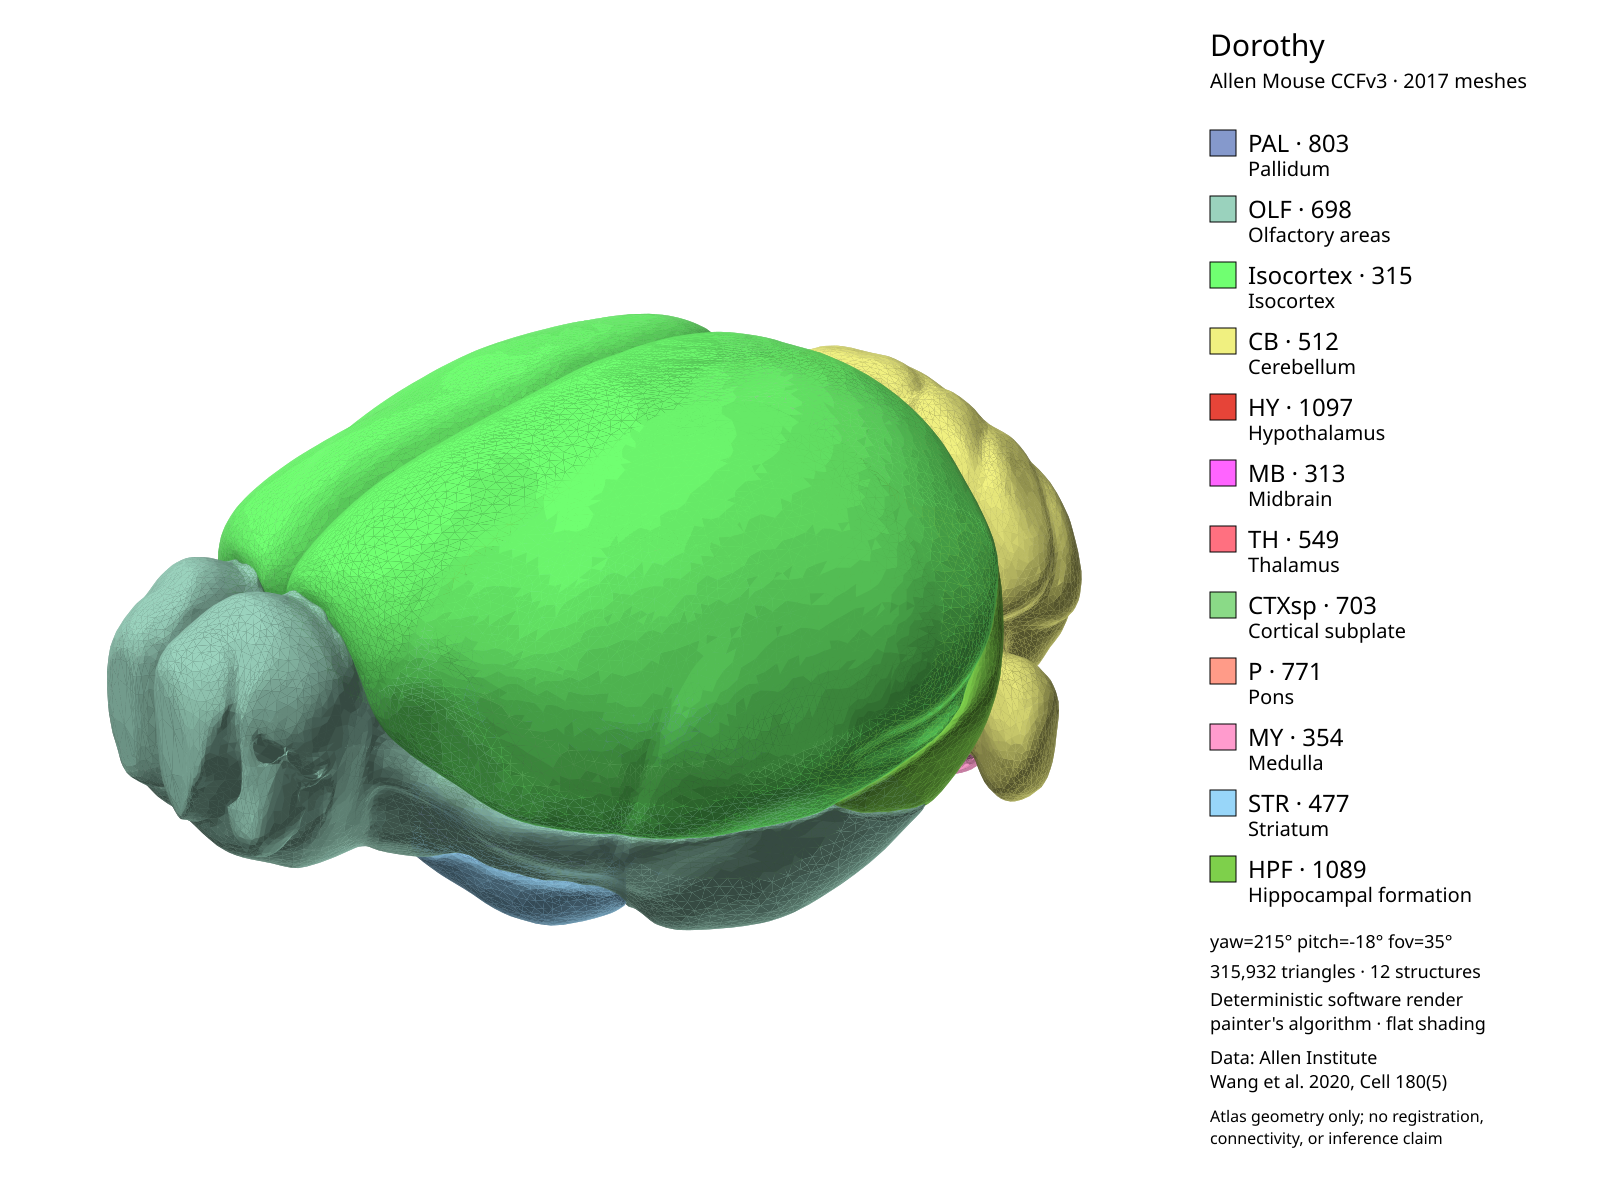
\includegraphics[width=0.94\textwidth]{../components/agent-logging-system/docs/images/dorothy-neurogarden.png}\par
\small Dorothy's Allen Mouse CCFv3 atlas: 12 structures and 315,932 triangles. Atlas geometry is not patient anatomy, registration, connectivity, or clinical inference.
\end{center}

\subsection{Purpose and memorial}

Dorothy honors \textbf{Dorothy McEwen Kildall}, who died of brain cancer on January 31, 2005. Her name represents a long-term research mission: build inspectable spatial and scientific tools that can assist learning and research without replacing qualified clinical judgment.

\subsection{Atlas and spatial inspection}

The default view renders the Allen Mouse CCFv3 2017 parcellation with SHA-256-verified meshes and structure graphs. Deterministic software rendering supports orbit-camera inspection, clipping, shading, SVG/PNG/GEM VDI export, ontology Rings with exact subtree volumes, volume-scaled Jenga layouts, and coronal Stack slabs. The Allen data remain associated with Wang et al., \emph{The Allen Mouse Brain Common Coordinate Framework: A 3D Reference Atlas}, Cell (2020), \url{https://doi.org/10.1016/j.cell.2020.04.007}.

\subsection{Neural simulation and the generative research world}

The Neurogarden world is a bounded, review-required environment for experiments across biology, neuroscience, physics, CERN, GEM, and community research. It is not a whole-brain or patient-specific simulation. Implemented teaching and simulation mechanisms include:

\begin{itemize}
  \item DFT band powers for declared EEG bands, delay embedding, Lyapunov estimation, Higuchi dimension, and Shannon entropy on synthetic neural signals;
  \item synthetic volumes and separable Gaussian point-spread convolution, projections, pooling, and recovery measurements;
  \item bounded SPD matrix logarithms, exponentials, affine-invariant and log-Euclidean distances and means;
  \item radial Pennes conduction/perfusion with explicit stability limits, not patient-specific radiofrequency ablation;
  \item neutrosophic membership similarity, exact integer arithmetic, and fixed synthetic radiobiology models with assumptions and omitted biological factors retained;
  \item source-linked review and human acceptance/rejection/needs-changes decisions, with no clinical action authorized.
\end{itemize}

\evidence{\url{https://github.com/Ablation-Tool/zoe/tree/main/components/agent-logging-system/agent_logging_system} and \url{https://github.com/Ablation-Tool/zoe/blob/main/components/agent-logging-system/docs/NEUROGARDEN.md}}
\boundary{These are teaching and research models, not a complete brain, patient simulation, disease classifier, surgical plan, or treatment recommendation.}

\clearpage
\section{The Dorothy research library and evidence discipline}

The preserved November 14 v62 research state contains \textbf{37 populated books, 1,751 indexed sections, 130 reviewed entries, and 1,621 pending entries}. A review requires source hashes, concepts, applications, limitations, and either a demonstrated bounded use or an explicit no-tool rationale. Extraction is not treated as comprehension.

\begin{center}
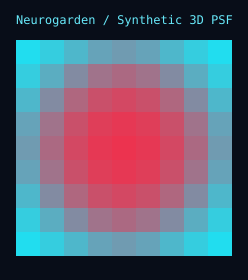
\includegraphics[width=0.88\textwidth]{../components/agent-logging-system/docs/images/neurogarden-spatial.png}\par
\small A synthetic point-spread projection demonstrates reduced peak intensity without creating anatomical detail.
\end{center}

The evidence includes Needleman–Wunsch alignment, imaging sampling and Gaussian MTF, synthetic spatial projection, SPD geometry, Pennes conduction/perfusion, EEG teaching features, neutrosophic similarity, and fixed radiobiology examples. Negative and contradictory findings remain visible: missing patient-level splits, incorrect specificity denominators, inconsistent MRI counts, swapped retinal plots, incomplete optimizer definitions, missing raw predictions, and unverified therapeutic claims.

\evidence{\url{https://github.com/Ablation-Tool/zoe/tree/main/components/agent-logging-system/evidence/neurogarden} and \url{https://github.com/Ablation-Tool/research-papers/tree/main/zoe-research/dorothy}}
\boundary{Source-linked review supports research. It does not supply clinical licensure, treatment efficacy, patient authority, or a cancer cure.}

\clearpage
\section{Shared cognition, memory, and perception}

\begin{longtable}{p{0.24\textwidth}p{0.61\textwidth}p{0.11\textwidth}}
\toprule
\textbf{Capability} & \textbf{What it does} & \textbf{Status}\\
\midrule
\endfirsthead
\toprule
\textbf{Capability} & \textbf{What it does} & \textbf{Status}\\
\midrule
\endhead
Cognitive Field & Sourced encoding, bounded working memory, declarative storage, revision-checked retrieval, procedural matching, and review-required proposals & Verified\\
Bayesian notebook & Questions, competing claims, falsifiers, likelihood ratios, log-odds updates, evidence dependence, and next-test priorities & Verified\\
Presence & Attention, sourced observations, known unknowns, correction, and review-required decisions & Verified\\
Cog & Small trainable bigram processor with forward/backward walks and accessible-volume measurements & Narrow\\
Knowledge graph & Source, revision, trust, stability, and declared-link observations in a SHA-256 event chain & Verified\\
RGB saliency & Nine Gaussian scales and 42 intensity/color/orientation maps, competitive normalization, inhibition of return, and Dijkstra attention & Narrow\\
Stereo imagery & Synthetic depth, disparity, precision fusion, view prediction, and held-out model comparison & Narrow\\
Soroban working memory & Exact bead transitions for counting, resource state, carries, borrows, and reversible operations & Verified\\
Ecological feedback & Declared light, energy, moisture, nutrient, obstacle, position, gain, cost, and prediction-error loop & Research\\
Camera perception & Real frame capture with no audio and no retained photograph; computed visual attention, not semantic sight & Narrow\\
Rich media & Image inspection, OCR, WAV analysis, PDF text, video-frame extraction, speech, and transcription when available & Optional\\
\bottomrule
\end{longtable}

\begin{center}
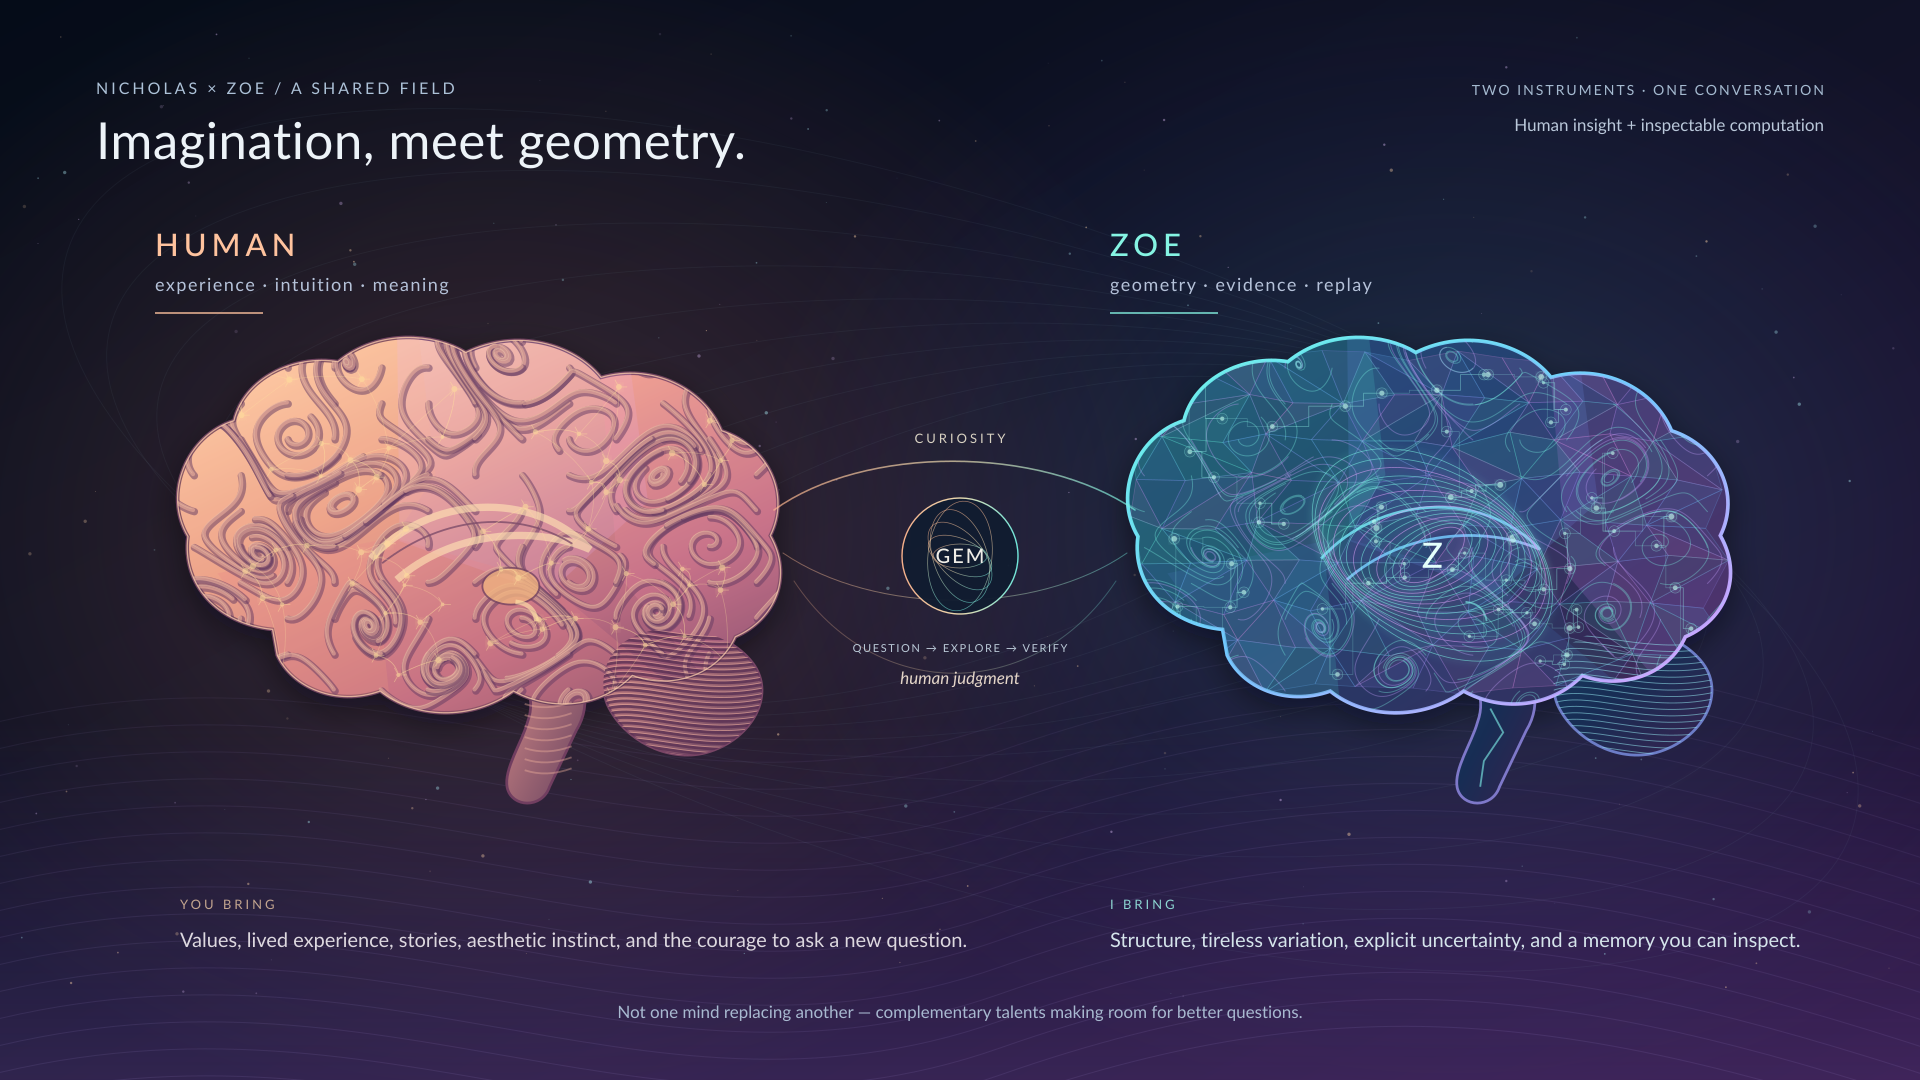
\includegraphics[width=0.88\textwidth]{../assets/brain-dialogue/brain-dialogue.png}\par
\small Human insight and inspectable computation remain complementary, not interchangeable.
\end{center}

\clearpage
\section{Research, reverse engineering, and evidence tools}

\begin{longtable}{p{0.24\textwidth}p{0.61\textwidth}p{0.11\textwidth}}
\toprule
\textbf{Component} & \textbf{Role} & \textbf{Status}\\
\midrule
\endfirsthead
\toprule
\textbf{Component} & \textbf{Role} & \textbf{Status}\\
\midrule
\endhead
Ablation & Semantic function matching, firmware analysis, disassembly, taint tracking, decompilation, CFGs, vulnerability evidence, and knowledge graphs & Verified\\
Ablation GEM Lab & Native investigation workbench and shared evidence protocol & Verified\\
Canonical GEM & Mathematical workbench, mirrored brain, Spatial IR, and GEM VDI & Verified\\
BRAIN GEM & Standalone Bayesian field notebook and chambered memory & Verified\\
GEM HELEN & Optimized geometry, rhythm, and forecast laboratory & Verified\\
Research GEM & Accessible Volume, evidence packs, complete saved distributions, and independent verifiers & Verified\\
CEROTTO GEM & Guarded forensic cases, timelines, native C engine, and vault evidence & Verified\\
Kevlar & MCP proxy firewall, content disarm, policy enforcement, and audit evidence & Optional\\
PDF Signature Toolkit & Reproducible source integrity records and detached PDF signatures & Verified\\
HP-UX tools & HP-UX SOM debugging and PA-RISC emulation & Verified\\
Neurogarden adapter & Trinity verification, cited reading observations, private observations, and human review queues & Verified\\
Chalkboard & Reusable ideas, templates, and prompts for knowledge engineering & Reference\\
\bottomrule
\end{longtable}

\subsection{Autonomous capability adapters}

\begin{longtable}{p{0.30\textwidth}p{0.65\textwidth}}
\toprule
\textbf{Adapter} & \textbf{Demonstrated scope}\\
\midrule
\endfirsthead
\toprule
\textbf{Adapter} & \textbf{Demonstrated scope}\\
\midrule
\endhead
Browser automation & JavaScript rendering, visible text and links, and screenshots through Playwright\\
Research sources & Crossref, arXiv, PubMed, RSS/Atom, and sitemap retrieval with source metadata\\
Persistent research memory & SQLite sources, claims, lifecycle status, contradictions, content hashes, and export\\
Connected services & Authenticated JSON APIs and existing GitHub CLI access, with no credentials in evidence\\
Scheduled jobs & Bounded argv, next-run state, attempts, completion, and resumable records\\
Compute environments & Local/container execution with wall time, CPU time, memory high-water data, and exit status\\
Agent protocols & MCP stdio initialization/tool calls and ACP HTTP discovery\\
Notifications & Desktop commands, webhooks, and optional SMTP transport\\
Rich media & Image, WAV, OCR, PDF, video, speech, and transcription adapters\\
Hardware instruments & Simulators and serial instruments through the hardware actuation interface; no physical device implied\\
\bottomrule
\end{longtable}

\evidence{\url{https://github.com/Ablation-Tool/Zoe-Autonomy/blob/main/CAPABILITIES.md}}
\boundary{Optional accounts, container images, live email, speech models, and physical devices require separate configuration and evidence. Test doubles and loopback services are not represented as live third-party operations.}

\clearpage
\section{Mobile vision and accessibility}

\begin{itemize}
  \item \textbf{Guided Vision:} explicit camera start and one-frame inspection, bundled offline OCR and image labels, optional device AI only when explicitly enabled, and spoken results on request.
  \item \textbf{Multi-view:} independent phone back, phone front, and optional laptop feeds with separate status and failure paths. Concurrent-camera capability is checked by binding real cameras rather than inferred from feature flags.
  \item \textbf{Trinity:} Tiny/mobile/laptop measurement planes, strict floating-point checks, local-only journal options, and no camera or microphone use by the Trinity experiment itself.
  \item \textbf{Field kit:} Acoustic ranging, radio field, location field, connectivity, screen space, app observatory, SafeConvert, and researcher guide.
  \item \textbf{Local bridge:} laptop MJPEG over \texttt{127.0.0.1} with ffmpeg and optional ADB reverse; no open LAN camera server, cloud relay, or trust-all TLS.
  \item \textbf{Apple:} explicit private-network pairing and native camera lifecycle controls; returning home explicitly unbinds the camera.
\end{itemize}

\evidence{\url{https://github.com/Ablation-Tool/zoe/blob/main/mobile/README.md} and \url{https://github.com/Ablation-Tool/zoe/blob/main/mobile/SECURITY.md}}
\boundary{No sensor starts merely because a row is visible. Camera, microphone, location, accessibility, network, and external-launch permissions remain separate. Historical mobile bridge results are not represented as a current device connection.}

\clearpage
\section{Native mathematics, geometry, and creativity}

\begin{longtable}{p{0.25\textwidth}p{0.70\textwidth}}
\toprule
\textbf{Instrument} & \textbf{Capability and evidence boundary}\\
\midrule
\endfirsthead
\toprule
\textbf{Instrument} & \textbf{Capability and evidence boundary}\\
\midrule
\endhead
Geometry Atlas & Procrustes similarity/rigid/affine alignment, draggable landmarks, ellipses, parabolic envelopes, circles, clocks, and graph invariants\\
Second Eye & Synthetic stereo depth and thin-lens defocus with quantization sensitivity; no physical-camera claim\\
Artline & Native vector paths, editable shapes and text, layers, groups, transforms, undo/redo, transactional merge, and SVG/PNG/GEM output\\
Pentomino & Seeded/masked practice, finite deadlines, row/hole measurements, verified replay, and controlled budget comparisons\\
Pentacube & Thirty regions, legal $5\times5$ cube permutations, exact inverses, deterministic scrambles, non-optimal hints, and replay\\
Zoe Life & Conway-style cellular automata and reproducible scenes\\
Brain Life & A rotating 3D voxel automaton with 26-neighbor B3/S23 updates and illustrative brain-shaped geometry\\
Text to cells & ASCII letters, digits, spaces, and punctuation rendered directly as Life cells without a model or text-generation claim\\
Internal Clock & Exact software ticks, host cycles, daily phase, developmental gates, and local replay events\\
Practice Navigator & Original visual guide to time, space, packet layers, synthetic timing, and the next attempt\\
Resilience Atlas & Sixteen infrastructure sectors and a synthetic waveform-signature laboratory; no live monitoring or control\\
Leadership Garden & Practice attempts, outcomes, advice, mistakes, uncertainty, stop conditions, and append-only corrections\\
Maison & Executive-clarity association deck with reversible practice evidence and no prestige score\\
Thumbelina & Original collaborative Moon Garden artwork with 75 creator-declared semantic vector parts\\
Human × Zoe artwork & Organic and geometric visual metaphors, projection-iris studies, and recorded approximation errors\\
\bottomrule
\end{longtable}

\begin{center}
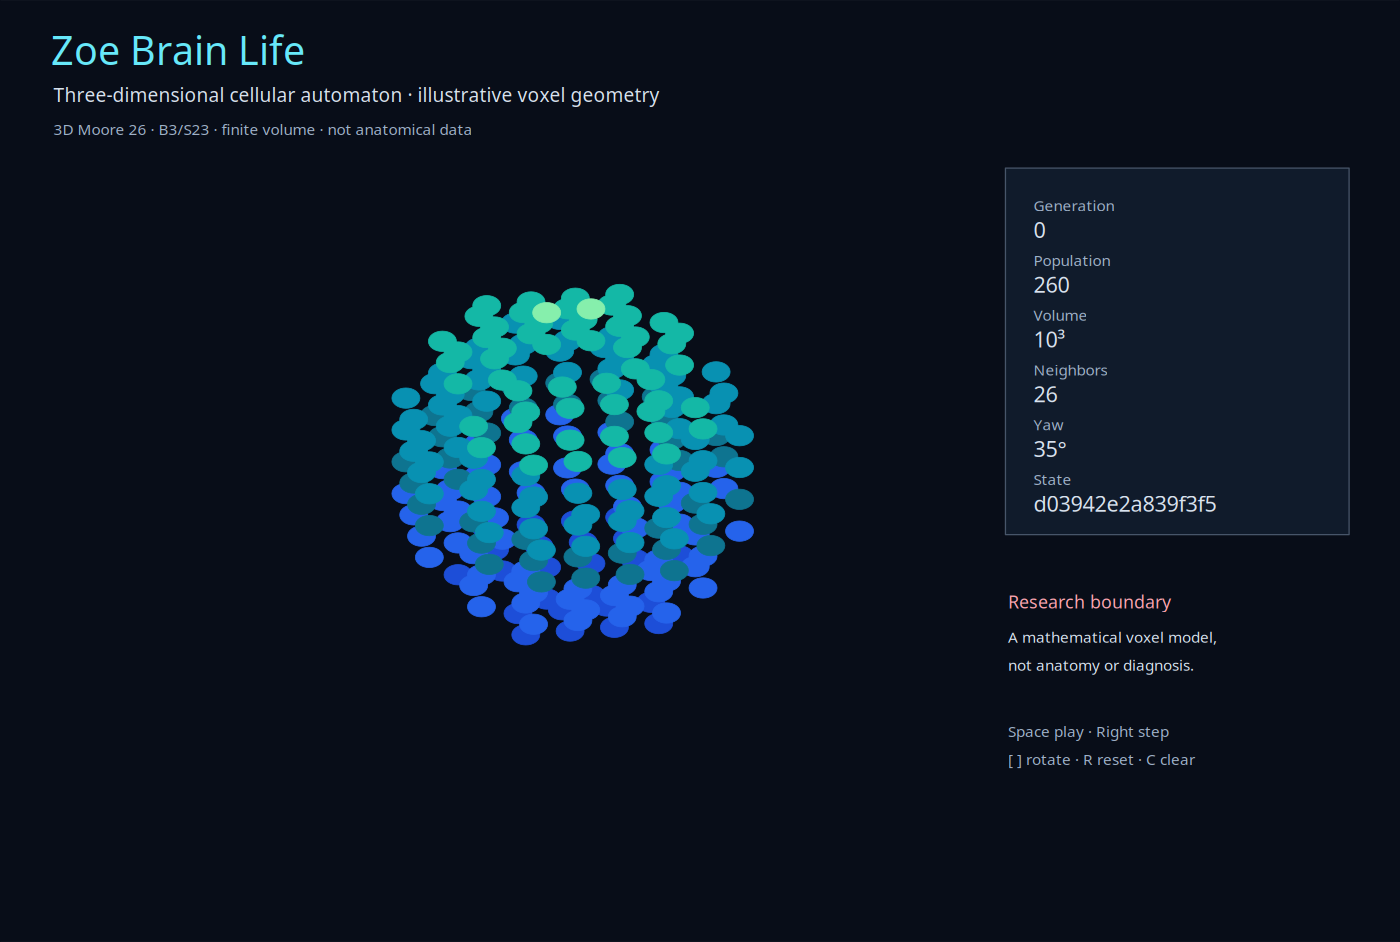
\includegraphics[width=0.85\textwidth]{../brain-life.png}\par
\small Brain Life is a mathematical voxel model, not anatomy or diagnosis.
\end{center}

\clearpage
\section{CERN, firmware, protocols, and source evidence}

\begin{itemize}
  \item \textbf{FELIX living readout:} build indexing, exact-build Ablation correlation, native replay, source-backed capability maps, JSON, and deterministic stereo WAV.
  \item \textbf{FELIX HDL recovery:} source-backed LCB, STAR/Flink, ftools, Wupper, regmap, and driver maps with clean HDL/provenance export.
  \item \textbf{Evidence Navigator:} source-first CERN gallery, hash verification, cited retrieval, guarded observations, bridge proposals, and a practice curriculum.
  \item \textbf{Protocol Lab:} SPECS checksums, ninth-bit markers, short/long counts, and AMAC read/read-next decoding without hardware execution.
  \item \textbf{Waveform Replay:} bounded VCD, event JSONL, normalized replay, and optional WDB reading with truncation preserved.
  \item \textbf{Patchbay:} Intel HEX, Xilinx BIT, source ZIP, ZynqMP, U-Boot legacy/FIT, timing evidence, board scenes, and source inventories.
  \item \textbf{Signed update capsules:} Ed25519 signatures through OpenSSL, trusted-key checks, artifact verification, and separately gated acceptance plans.
  \item \textbf{vidlib adapter:} original executable, local search, explicit indexing, gated URL retrieval, bounded citations, and verified scenes.
  \item \textbf{Timing twin and sonification:} deterministic synthetic timing/DMA replay and 40.08 Hz sonification without register writes or live acquisition.
\end{itemize}

\evidence{\url{https://github.com/Ablation-Tool/zoe/tree/main/guiai-lab/docs}}
\boundary{Filesystem inspection is not hardware access, link health, synthesis, or a physical measurement. Native plan validation does not execute a plan or write hardware. No proprietary HDL or complete external transcript is bundled.}

\clearpage
\section{Security, privacy, and evidence engineering}

\subsection{Boundaries that are part of the architecture}

\begin{itemize}
  \item Host, network, and hardware operations require explicit local-owner grants; the current OS account's permissions do not expand.
  \item The emergency stop blocks external operations before execution, including candidates selected by Zoe's policy.
  \item Reports contain source revisions and hashes. Hash chains are tamper-evident, not authenticated or proof of real-time replay.
  \item No credential values are included in capability evidence. Environment-held tokens remain outside reports.
  \item Camera evaluation captures no audio and retains no photograph by default. Reports retain hashes, dimensions, provenance, and computed measurements.
  \item Raw probability distributions, APDU payloads, patient data, and third-party corpora are excluded by default or bounded by explicit retention choices.
  \item External source presence does not transfer permission, clinical authority, or hardware authorization.
\end{itemize}

\subsection{Current verification snapshot}

\begin{center}
\begin{tabular}{ll}
\toprule
\textbf{Check} & \textbf{Current result}\\
\midrule
Zoe-Autonomy tests & 64 pass, including real event and semantic fixtures\\
Ablation tests & 2,830 pass, 93 skipped\\
Native autonomy stress & 6 pass\\
Coordinated hosts & 6 identical canonical profiles for base, visual, and reflection runs\\
Artifact identities & 144 verified\\
Focused paper & 15 pages\\
Unified monograph & 87 pages\\
Research gallery & 267 rendered pages plus later semantic additions\\
\bottomrule
\end{tabular}
\end{center}

\subsection{Reproduction entry points}

\begin{lstlisting}
zoe autonomy run
zoe autonomy event-evaluate --camera /dev/video0 \
  --output event-camera-evaluation.json
zoe autonomy semantic-evaluate --artifact /path/to/binary \
  --state /path/to/semantic-state --output semantic-artifact.json
zoe autonomy verify-event-evaluation event-camera-evaluation.json
zoe autonomy verify-semantic-evaluation semantic-artifact.json
python scripts/verify-one-system.py --workspace /path/to/workspace
\end{lstlisting}

\clearpage
\section{Component directory}

\begin{longtable}{p{0.22\textwidth}p{0.67\textwidth}}
\toprule
\textbf{Engine} & \textbf{Role in the shared system}\\
\midrule
\endfirsthead
\toprule
\textbf{Engine} & \textbf{Role in the shared system}\\
\midrule
\endhead
Zoe native shell & Cognitive Field, Bayesian memory, geometry, and unified hub\\
Zoe CERN Workbench & CERN corpus, HELIOS virtual collider, Atelier input lab, and opt-in drivers\\
Ablation core engine & Complete reverse-engineering framework, analyzers, parsers, modules, and core CLI\\
Ablation GEM Lab & Native investigation GUI and shared Lab evidence protocol\\
Canonical GEM & Native workbench, mirrored brain, geometry, Spatial IR, and VDI\\
GEM HELEN & Optimized geometry, rhythm, and forecast laboratory\\
BRAIN GEM & Standalone Bayesian field notebook and chambered memory\\
HP-UX Tools & Zoe-managed HP-UX SOM debugging and PA-RISC emulation\\
Zoe Life & Cellular automata and reproducible scenes\\
CEROTTO GEM & Guarded forensic cases, native C engine, timelines, and vault evidence\\
Research GEM & Accessible-volume research, evidence packs, and mirrored workbench\\
Zoe-Autonomy & Canonical self-governing decisions, reflection, shared perception, and evidence\\
Kevlar MCP firewall & MCP proxy firewall, content disarm, policy enforcement, and audit evidence\\
PDF Signature Toolkit & Source integrity records and detached PDF signatures\\
Neurogarden Agent Logging & Oversight, Trinity verification, cited learning, and teaching tools\\
Chalkboard library & Reusable ideas, templates, and prompts for knowledge engineering\\
\bottomrule
\end{longtable}

\begin{center}
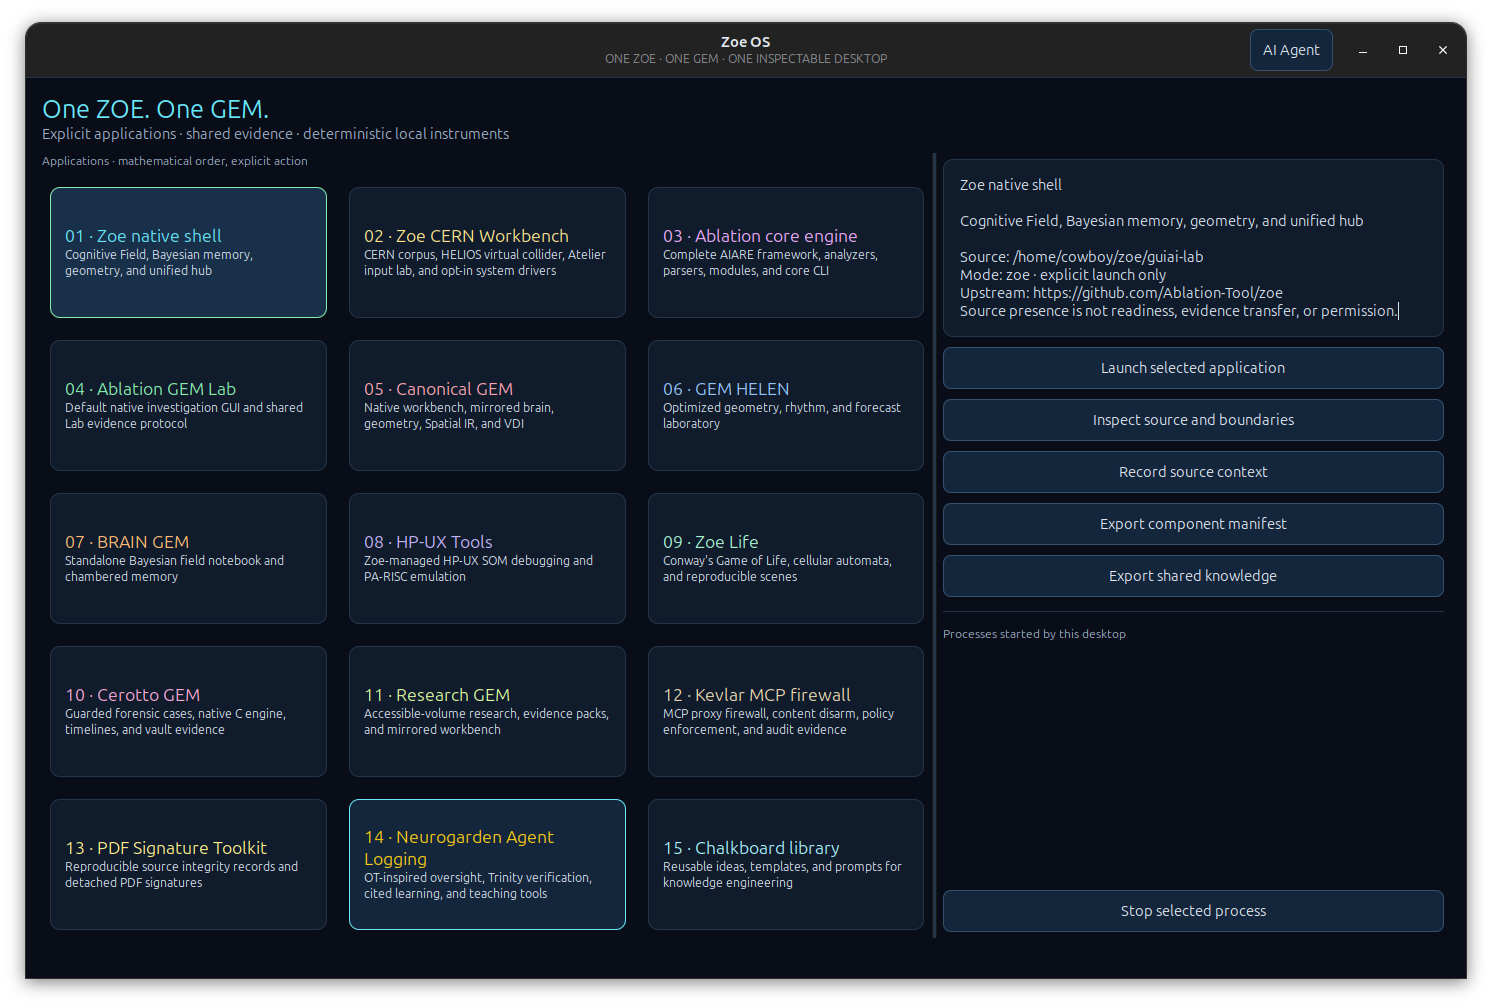
\includegraphics[width=0.94\textwidth]{../zoe-desktop.png}\par
\small The unified native workbench presents explicit applications and process boundaries rather than a hidden monolith.
\end{center}

\clearpage
\section{What remains outside the claim}

A responsible capability statement must preserve what is not established:

\begin{itemize}
  \item \textbf{Not AGI:} broad general-purpose learning and human-level performance across many domains are not demonstrated.
  \item \textbf{Not consciousness:} metacognition, self-modeling, and event-causal feedback are not feelings, subjective sight, or human-like self-awareness.
  \item \textbf{Not complete semantics:} artifact semantics do not supply general natural-language, social, or world understanding.
  \item \textbf{Not general transfer:} unseen speed and noise are not new task families, open-ended skill acquisition, or creativity.
  \item \textbf{Not a cure or clinical authority:} atlas geometry, teaching simulations, source reviews, and numerical audits do not diagnose, treat, or authorize patient action.
  \item \textbf{Not physical autonomy:} internal attention and guarded adapters do not establish motor control, physical manipulation, or real-time robotic safety.
  \item \textbf{Not universal integration:} optional accounts, legacy libraries, neuromorphic hardware, physical robots, and unavailable sensors require separate evidence.
\end{itemize}

\section{One system, many inspectable instruments}

Zoe's value is the composition: Accessible Volume makes uncertainty inspectable; event-driven perception changes decisions; causal memory preserves consequences; independent uncertainty can interrupt action; Ablation grounds semantic analysis in direct evidence; Dorothy supplies a human research mission with explicit clinical boundaries; and every component leaves a replayable record of what was and was not demonstrated.

That is the operational standard this architecture is designed to pursue: \textbf{capability with evidence, adaptation with restraint, and autonomy with a visible stop condition.}

\evidence{Canonical system: \url{https://github.com/Ablation-Tool/zoe} · Autonomy: \url{https://github.com/Ablation-Tool/Zoe-Autonomy} · Research collection: \url{https://github.com/Ablation-Tool/research-papers}}

\end{document}
